\chapter{Resultados del Proyecto}

\section{Comparación de las predicciones hechas con el nuevo módulo con las predicciones hechas con el anterior método } \label{subsec:ComparacionesNuevoYviejoMetodo}

La gráfica \ref{fig:GraficaEstadisticas} muestra dos predicciones, la gráfica de azul es la predicción del nuevo módulo de predicción, y la gráfica verde es la predicción hecha con el método anterior (de la competencia 2016), podemos observar que la predicción hecha con el nuevo módulo es evidentemente mejor, y el resultado de sus respectivos errores medios absolutos lo confirma, pero la gráfica \ref{fig:GraficaEstadisticas} solo muestra la predicción en el timeslot 385, con forme avanzan los timeslots el método anterior de promedios ponderados mejora su predicción, por ejemplo la predicción hecha en el timeslot 830 por este método anterior, mostrada en la gráfica de la figura \ref{fig:comparacionNuevoConAnterior1agente}, fue mejor que en el timeslot 385, y casi alcanza a la predicción hecha con el nuevo método (mostrada en azul). Para medir cuan mejor fue en todo el juego, se ocupo la función \textit{Calcular error global} (explicado en la sección \ref{subsec:menuEstadisticas}) y este arrojó como error global del la predicción del nuevo método 3565.4893, y para el anterior 4424.4641, como se ve en el título de la ventana de la figura \ref{fig:comparacionNuevoConAnterior1agente}, esto representa una mejora del 20\% (el error disminuyó un 20\%)en la predicción, lo cual no representa mucho para la competencia real, ya que esta prueba se hizo con el agente corriendo con el default broker únicamente, así que no hubo las interferencias que estos producen, y que este nuevo módulo tiene en cuenta.

\begin{figure}[h]
	\centering
	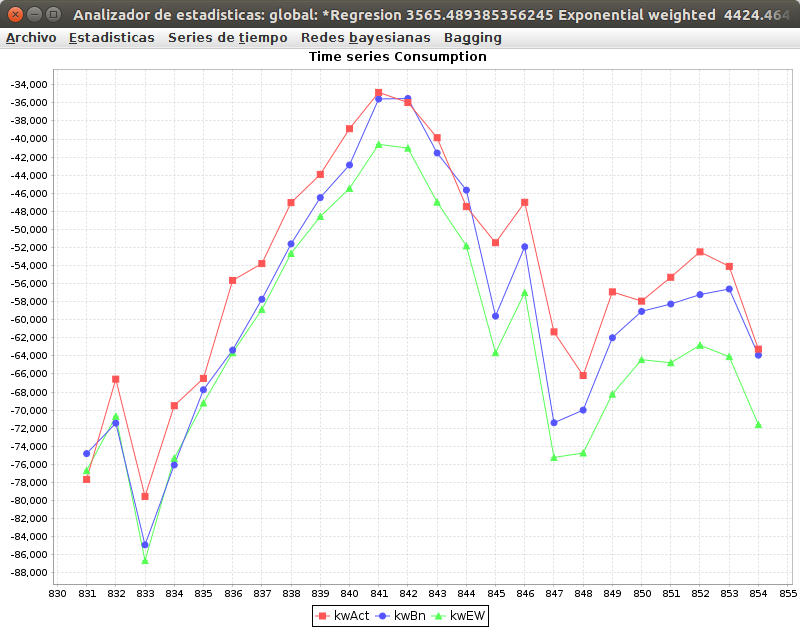
\includegraphics[width=12cm]{img/comparacionNuevoConAnterior1agente.png}
	\caption{Predicciones de balance del timeslot 830 y resultado global. }
	\label{fig:comparacionNuevoConAnterior1agente}
\end{figure}

La verdadera mejora fue el hecho de que el nuevo módulo de predicción se adapta a la pérdida o ganancia constante de clientes, lo cual no hace el método anterior, en la figura \ref{fig:comparacionNuevoConAnterior3agentes} podemos ver una gráfica con los resultados de predicción de balance en un juego donde participaron los agentes Maxon y AgentUDE, donde la fluctuación en el numero de clientes afecta la predicción, en este caso, unos timeslots atrás había menos clientes, por lo que el cálculo del método anterior, el cual hizo el promedio ponderado para cada hora con estos valores,  fue inferior al real, mientras que la predicción del nuevo método (en azul) se adaptó mejor a estos cambios, dando un error medio absoluto global de 2738.3087, mientras que en la predicción con el método anterior (en verde) tuvo un error medio absoluto global de 4794.6719, lo cual representa una mejora significativa del 43\%.

\begin{figure}[h]
	\centering
	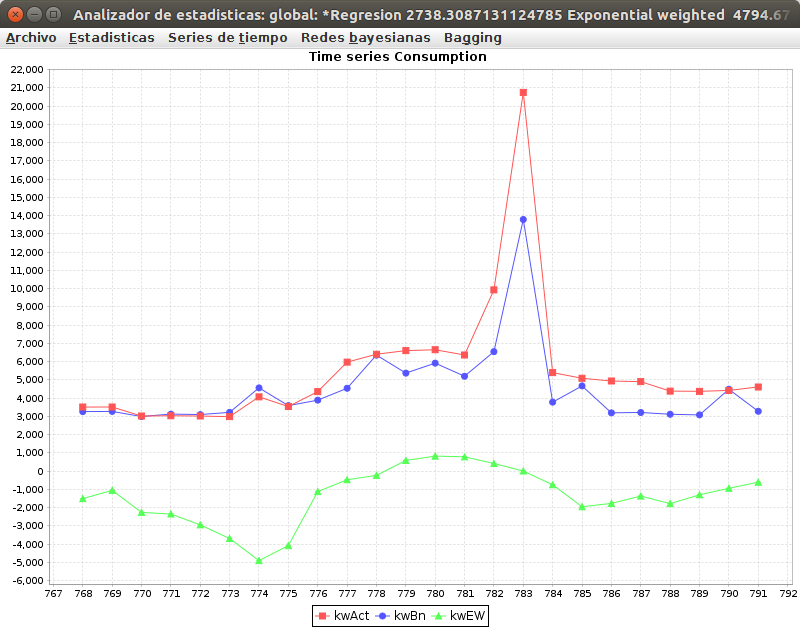
\includegraphics[width=12cm]{img/comparacionNuevoConAnterior3agentes.png}
	\caption{Predicciones de balance del timeslot 830 y resultado global. }
	\label{fig:comparacionNuevoConAnterior3agentes}
\end{figure}
\clearpage
\section{Participación en la competencia PowerTAC2017} \label{subsec:participacionComp}

La competencia Power TAC 2017 consistió en dos rondas de prueba llamadas trial 1 y trial 2 de los días 27 al 31 de marzo y 18 al 15 de abril respectivamente, una ronda clasificatoria del 15 al 19 de mayo y una ronda final del 12 al 21 de junio. 
Las rondas trial tienen el objetivo de que los participantes puedan probar sus agentes antes de que las rondas clasificatoria y final comiencen para que puedan hacer los ajustes necesarios y depurar cualquier error, puesto que correr un agente contra el default broker únicamente tiene resultados diferentes tal como se vio en la sección \ref{subsection:pruebasDefaultBrokerMaxonYUDE}, es por esto que los resultados no se publicaron.

En esta competencia participaron equipos de 8 universidades, los participantes son:

\begin{table}[h!]
	\centering
	%\scalebox{0.9}{
	\begin{tabular}{|p{2.76cm}|p{8cm}|p{5.4cm}|} \hline
		\textbf{Agente}	 		& \textbf{Institución} 			& \textbf{Encargados} \\\hline	
	    AgentUDE	 	& Universitaet Duisburg-Essen / DAWIS 	& Serkan Ozdemir \\\hline	
    	COLDPower17		& INAOE									& Ansel Y. Rodríguez González\\\hline	
	    CrocodileAgent	& University of Zagreb					& Jurica Babic	\\\hline	
	    SPOT			& UTEP/NMSU								& Chris Kiekintveld\\\hline	
	    VidyutVanika	& IIIT Hyderabad (Machine Learning Lab) TCS & Susobhan Ghosh\\\hline	
	    ewiBroker		& Institute of Energy Economics at the University of Cologne & Martin Paschmann\\\hline	
    	fimtac			& Universität Augsburg, TU München, Universität Bayreuth& Carina Antonin, Lea Jäntgen, Moritz Wöhl\\\hline	
	    maxon17			& Westfaelische Hochschule				& Tobias Urban \\\hline
	\end{tabular}
	%}
\caption{Tabla de participantes de la competencia Power TAC 2017}
\end{table}

Las rondas consisten en 60 juegos donde participan los 8 agentes, 112 juegos en los que participan 5 agentes(todas las posibles combinaciones de 5 en 8 dos veces) y 112 juegos en los que solo participan 3 agentes (las combinaciones de 5 en 3 dos veces), cada juego es una simulación de aproximadamente 2 horas de duración, en las que se simulan 2 meses de eventos en un mercado energético (se simula una hora cada 5 segundos, esto es un timeslot). Estos juegos se simulan uno tras otro (con pausas de pocos segundos) en el lapso hasta que terminen los juegos, esto suele durar varios días. Durante este tiempo los equipos tienen permitido cambiar parámetros en los agentes, pero no se puede cambiar código. 

Durante la rondas de clasificación 
el Dr. Ansel (asesor externo de este proyecto y líder del equipo de programación) se dio cuenta de algo que generalmente ocurría, la red estaba balanceada negativamente (había mas consumo que producción), esto permitía seguir una estrategia de mercadeo que por lo general funcionaba, esta consistía en comprar energía en el mercado al por mayor, asegurándose que el desbalance siempre sea positivo, debido a que el sistema recompensa a los brokers que aportan balance a la red (y la red esta generalmente balanceada negativamente), y esta ganancia extra hacia posible pagar la energía comprada en el mercado al por mayor teniendo ganancias en la mayoría de los casos.

Esta estrategia se implemento en la ronda final, y dio muy buenos resultados en los primeros juegos, el agente COLDPower ganaba millones, pero después de cierta cantidad de juegos los organizadores de la competencia se dieron cuenta y decidieron cambiar la configuración y reiniciar los juegos, esto hizo que el aprendizaje que tuvieron los expertos durante los juegos anteriores ya no resultara bueno para esta nueva configuración, lo que significó muchas pérdidas para los agentes COLDPower y SPOT, que estaban usando la estrategia mencionada.
Después de que esta configuración fue cambiada y ver que se perdía mucho dinero con la estrategia implementada, se utilizó una estrategia secundaria, en la cual se compraba energía en el mercado de tarifas (mas inestable), así que el broker ya no perdía tanto dinero, pero aun perdía por las penalizaciones de desbalance, esto debido a que la configuración que tenía, hacia muy difícil tener ganancias, la mayoría de los agentes tenían pérdidas, la mejor estrategia era no hacer nada, por lo que se quedaría en 0 y habría quedado en segundo lugar, justo debajo de AgentUDE, puesto que los demás quedaron en números negativos.

Al final el agente COLDPower logró recuperarse un poco de las pérdidas que generó la primera estrategia, quedando en sexto lugar con los resultados mostrados en la figura \ref{fig:resultadosCompetencia}, esta tabla muestra los resultados por cada uno de los tipos de juegos (de 8, 5 y 3 agentes) y el total.

\begin{figure}[h]
	\centering
	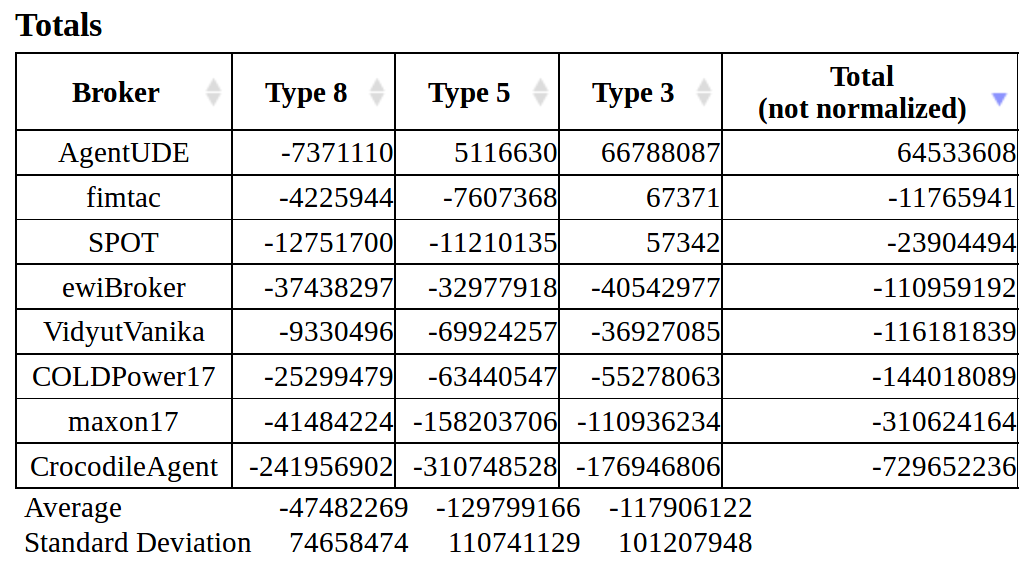
\includegraphics[width=17cm]{img/resultadosCompetencia.png}
	\caption{Resultados de la competencia PowerTAC 2017. }
	\label{fig:resultadosCompetencia}
\end{figure}
